\subsection{Principles of Data Collection} \label{sec:DC}
\begin{tcolorbox}[title=Fisher's Maxim]
To consult the statistician after an experiment is finished is often merely to ask him to conduct a post mortem examination. He can perhaps say what the experiment died of. \\[-0.6cm]
\begin{flushright}
-- R.A. Fisher, Presidential Address to the \textit{First Indian Statistical Congress}, 1938
\end{flushright}
\end{tcolorbox}
\noindent Data analysis tools and techniques work in conjunction with collected data. The type of data that needs to be collected to carry out such analyses, as well as the priority placed on the collection of quality data relative to other demands, will dictate the choice of data collection strategies. The manner in which the resulting outputs of these analyses are used for decision support will, in turn, influence appropriate data presentation strategies and system functionality (we will revisit this aspect in a later section).  
\newl Although consultants should always endeavour to work with \textbf{representative} and \textbf{unbiased data}, there will be times when the available data is flawed and not easily repaired. Quantitative consultants have a professional responsibility to explore the data, looking for potential fatal flaws \textbf{prior} to  the start of the analysis and to inform their client of any findings that could halt, skew, or simply hinder the analytical process or its applicability to the situation at hand. 
\par Unless a clause has specifically been put in the contract to allow a graceful exit at this point, you will have to proceed with the analysis, flaws and all. It is  \textbf{EXTREMELY IMPORTANT} that you do not simply sweep these flaws under the carpet. Address them repeatedly in your meetings with the clients, and make sure that  the analysis results you present or report on include an appropriate \textit{caveat}. \paragraph{Data Collection System} Consultants might also be called upon to provide suggestions to evaluate or fix the data collection system. The following items could help with that task. 
\begin{itemize}[noitemsep]
\item \textbf{Data Validity}: the system must collect the data in such a way that data validity is ensured during initial collection. In particular, data must be collected in a way that ensures sufficient accuracy and precision of the data, relative to its intended use.
\item \textbf{Data Granularity, Scale of Data}: the system must collect the data at a level of granularity appropriate for future analysis.
\item \textbf{Data Coverage}: the system must collect data that comprehensively, rather than only partially or unevenly, represents the objects of interest. As well, the system must collect and store the required data over a sufficient amount of time, and at the required intervals, to support data analyses that require data spanning a certain duration.
\item \textbf{Data Storage}: the system must have the functionality to store the types and amount of data required for a particular analysis.
\item \textbf{Data Accessibility}: the system must provide access to the data relevant for a particular analysis, in a format that is appropriate for this analysis.
\item \textbf{Computational/Analytic Functionality}: the system must have the ability to carry out the computations required by relevant data analysis techniques.
\item \textbf{Reporting, Dashboard, Visualization}: the system must be able to present the results of the data analysis in a meaningful, usable and responsive fashion.
\end{itemize}
\newpage\noindent A number of different overarching strategies for data collection can be employed. Each of these different strategies will be more or less appropriate under certain data collection circumstances, and will result in different system functional requirements. In this section we will focus on survey sampling, questionnaire design, and automated data collection. 
\begin{center}
    \rule{0.5\textwidth}{.4pt}
\end{center}
\paragraph{Formulating the Problem} The \textbf{objectives} drive all other aspects of quantitative analysis. With a \textbf{question} (or questions) in mind, an investigator can start the process that leads to \textbf{model selection}. With potential models in tow, the next step is to consider what \textbf{variates} (fields, variables) are needed, the \textbf{number} of observations required to achieve a  pre-determined \textbf{precision}, and how to best go about \textbf{collecting}, \textbf{storing} and \textbf{accessing} the data.\newl Another important aspect of the problem is to determine whether the questions are being asked of the data in and of \textbf{itself}, or whether the data is used as a \textbf{stand-in for a larger population}. In the later case, there are other technical issues to incorporate into the analysis in order to be able to obtain generalizable results.  
\newl Questions do more than just drive the other aspects of data analysis -- they also drive the development of quantitative methods. They come in all flavours and their variability and breadth make attempts to answer them challenging: no single approach can work for all of them, or even for a majority of them, which leads to the discovery of better methods, which are in turn applicable to new situations, and so on, and so on.  
\newl 
Not every question is answerable, of course, but a large proportion of them may be answerable partially or completely; quantitative methods can provide insights, estimates and ranges for possible answers, and they can point the way towards possible implementations of the solutions.
\newl As an example, consider the following questions.
\begin{itemize}[noitemsep]
\item Is cancer incidence higher for second-hand smokers than it is for smoke-free individuals? 
\item Using past fatal collision data and economic indicators, can we predict future fatal collision rates given a specific national unemployment rate?   
\item What effect would moving a central office to a new location have on average employee commuting time?  
\item Is a clinical agent effective in the treatment against acne?
\item Can we predict when border-crossing traffic is likely to be higher than usual, in order to appropriately schedule staff rotations? 
\item Can personalized offers be provided to past clients to increase the likelihood of them becoming repeat customers? 
\item Has employee productivity increased since the company introduced mandatory language training?   
\item Is there a link between early marijuana use and heavy drug use later in life? 
\item How do selfies from over the world differ in everything from mood to mouth gape to head tilt?
\end{itemize}
\noindent How can such questions be answered? In many instances, the next step requires obtaining data.   
\newpage\noindent 
\paragraph{Data Types} 
Data has \textbf{attributes} and \textbf{properties}. Fields are classified as \textbf{response}, \textbf{auxiliary}, \textbf{demographic} or \textbf{classification} variables; they can be \textbf{quantitative} or \textbf{qualitative}; \textbf{categorical}, \textbf{ordinal} or \textbf{continuous}; \textbf{text-based} or \textbf{numerical}. \par Data is \textbf{collected} through experiments, interviews, censuses, surveys, sensors, scraped from the Internet, etc. 
\begin{center}
    \rule{0.5\textwidth}{.4pt}
\end{center} Collection methods are not always sophisticated, but new technologies usually improves the process in many ways (while introducing new issues and challenges): modern data collection can occur over one pass, in batches, or continuously.
\par How does one decide which data collection method to use? The type of question to answer obviously has an effect, as do the required precision, cost and timeliness. Statistics Canada's \textit{Survey Methods and Practices} provides a wealth of information on probabilistic sampling and questionnaire design, which remain relevant in this day of big (and real-time) data. \newl A full discussion on the various collection methods currently available is outside the scope of this section, but the importance of this step cannot be overstated: without a well-designed plan to collect meaningful data, and without safeguards to identify flaws (and possible fixes) as the data comes in, subsequent steps are likely to prove a waste of time and resources. \begin{center}
    \rule{0.5\textwidth}{.4pt}
\end{center}
As an illustration of the potential effect that data collection can have on the final analysis results, contrast the two following ways to collect similar data on two different populations.
\begin{tcolorbox}[title=Yes. I Mean No. ... I Think.]
The Government of Qu\'ebec has made public its proposal to negotiate a new agreement with the rest of Canada, based on the equality of nations; this agreement would enable Qu\'ebec to acquire the exclusive power to make its laws, levy its taxes and establish relations abroad $-$ in other words, sovereignty $-$ and at the same time to maintain with Canada an economic association including a common currency; any change in political status resulting from these negotiations will only be implemented with popular approval through another referendum; on these terms, do you give the Government of Qu\'ebec the mandate to negotiate the proposed agreement between Qu\'ebec and Canada? \\[-0.6cm]
\begin{flushright}
-- 1980 Qu\'ebec sovereignty referendum question
\end{flushright}
\end{tcolorbox}
\begin{tcolorbox}[title=Do You Think They Learned Something From 1980?]
Should Scotland be an independent country? \\[-0.6cm]
\begin{flushright}
-- 2014 Scotland independence referendum question
\end{flushright}
\end{tcolorbox}
\noindent The end result was the same in both instances, but arguments can be made that the Scottish `No` was a much clearer `No` than the Qu\'ebec `No` of 34 years earlier -- in spite of the smaller 2014 victory margin (55.3\%-44.7\%, as opposed to 59.6\%-40.4\%). 
\newpage\noindent
\paragraph{Data Storage and Access}
Data \textbf{storage} is also strongly linked with the data collection process, in which decisions need to be made to reflect how the data is being collected (one pass, batch, continuously), the volume of data that is being collected, and the type of access and processing that will be required (how fast, how much, by whom).\par Stored data may go \textbf{stale} (e.g. people move, addresses no longer accurate), so it may be necessary to implement regular updating collection procedures. 
\newl 
Until very recently, the story of data analysis has been written for small datasets: useful collection techniques yielded data that could, for the most part, be stored on personal computers or on small servers. The advent of Big Data has introduced new challenges \textit{vis-\`a-vis} the collection, capture, access, storage, analysis and visualisation of datasets; some effective solutions have been proposed and implemented, and intriguing new approaches are on the way (such as DNA storing, to name but one). We shall not discuss those challenges in detail, but be aware of their existence.  

\subsubsection{Questionnaire Design}
\begin{tcolorbox}[title=A Modern Paradox]
People resist a census, but give them a profile page and they'll spend all day telling you who they are. \\[-0.6cm]
\begin{flushright}
-- Max Berry, \textit{Lexicon}, 2013
\end{flushright}
\end{tcolorbox}
\noindent 
A \textbf{questionnaire} is a sequence of questions designed to obtain information on a subject from a respondent. Design principles vary according to the subject matter and the mode of data collection, but we strongly encourage pre-testing a variety of questionnaires.\paragraph{Questionnaire Design Basics} In general, questionnaires should: 
\begin{itemize}[noitemsep] 
\item be as brief as possible, with no wasted questions;
\item be accompanied by clear and concise instructions;
\item keep the respondent's interests in mind;
\item emphasise confidentiality;
\item be serious and courteous in tone;
\item be free of mistakes and laid out attractively;
\item be worded clearly; 
\item be designed to be accurately answered, and 
\item be ordered attentively. 
\end{itemize}
\paragraph{Question Types} The basic questionnaire unit is, of course, the \textbf{question}, which comes in two flavours: 
\begin{itemize}[noitemsep]
\item \textbf{closed}, with a fixed number of pre-determined mutually exclusive and collectively exhaustive answer choices (and should always include an ``Other (Please Specify)'' category to counteract the loss of expressiveness of such questions), and
\item \textbf{open}, which serves to identify common response choices to be used as closed question choices in subsequent questionnaires. 
\end{itemize}
\paragraph{Wording Considerations} It is well known that the wording of the questions can influence a questionnaire's responses \cite{DC_G}; please keep the following \textbf{wording considerations} in mind when designing a questionnaire:   
\begin{itemize}[noitemsep] 
\item avoid \textbf{abbreviations} and \textbf{jargon} (``Does your organization use any TTWQ practices?'');
\item do not use words and terminology that are \textbf{too complex} (``How often have you been defenestrated?'' vs.\@ ``How often have you been thrown out of a window?'');
\item specify the \textbf{frame of reference} (``What is your income?'' vs.\@ ``What was your household's total income form all sources before taxes and deductions in 2017?'');
\item make the question as \textbf{specific} as possible (``How much fuel did your moving company use during the last year?'' vs.\@ ``How much did your moving company  spend on fuel during the last year?'');
\item ensure that the questions can be answered by all respondents;
\item avoid \textbf{double-barrelled} questions (``Do you plan to leave your car at home and take the bus to work during the coming year?''), and 
\item avoid leading questions (see the always excellent \cite{DC_YPM} for a not-so-facetious example).
\end{itemize}
\paragraph{Question Order} The order of the questions is just as important as the wording. Questionnaires should be designed to \textbf{flow smoothly} and \textbf{follow a logical sequence} (logical to the respondent, that is).  
\begin{enumerate}[noitemsep]
\item Start with an \textbf{introduction} which provides the title, subject, and purpose of the survey.
\item Request \textbf{cooperation} and explain the importance of the survey and how the results will be used.
\item Indicate the degree of \textbf{confidentiality} and provide a deadline and a contact address.
\item Open with a series of \textbf{easy} and \textbf{interesting questions} to establish the respondent's confidence.
\item Group similar questions under a \textbf{common heading}.
\item Introduce \textbf{sensitive topics} once trust and confidence are likely to have developed.
\item Allow some space and/or time for \textbf{additional comments}.
\item \textbf{Thank} the respondent for their participation.
\end{enumerate}
\begin{center}
    \rule{0.5\textwidth}{.4pt}
\end{center}
A lot more has been written about questionnaire design (see \cite{DC_O}, for instance). It can be surprisingly easy to get lost in the jungle and spend way too much time on the ``perfect'' design; remember that without a sound sampling plan, whatever data is collected may not prove up to the task of drawing the actionable insights that the client is really interested in seeing  answered. 
\subsubsection{Automated Data Collection}\label{sec:adc}
\begin{tcolorbox}[title=One Man's Trash...]
It's been said that the streets of the Web are paved with data that cannot wait to be collected, but you'd be surprised at how much trash there is out there. \\[-0.6cm]
\begin{flushright}
-- Patrick Boily, 2018
\end{flushright}
\end{tcolorbox}
\noindent The way we \textbf{share}, \textbf{collect}, and \textbf{publish} data has changed over the past few years due to the ubiquity of the \textit{World Wide Web}. \textbf{Private businesses}, \textbf{governments}, and \textbf{individual users} are posting and sharing all kinds of data and information. At every moment, new channels generate vast amounts of data.

There was a time in the recent past where both scarcity and inaccessibility of data was a problem for researchers and decision-makers. That is \textbf{emphatically} not the case anymore. 
\newl Data abundance carries its own set of problems, however, in the form of 
\begin{itemize}[noitemsep]
\item tangled masses of data, and 
\item traditional data collection methods and classical (small) data analysis techniques not being up to the task anymore. 
\end{itemize}
The growth and increasing popularity and power of \textbf{open source software}, such as \textit{R} and \textit{Python}, for which the source code can be inspected, modified, and enhanced by anyone, makes program-based automated data collection quite appealing. 

One note of warning, however: time marches on and packages become \textbf{obsolete} in the blink of an eye. If the analyst is unable (or unwilling) to \textbf{maintain their extraction/analysis code} and to \textbf{monitor the sites} from which the data is extracted from, the choice of software will not make much of a difference. 
\begin{center}
    \rule{0.5\textwidth}{.4pt}
\end{center}
So why bother with automated data collection? Common considerations include:
\begin{itemize}[noitemsep]
    \item the sparsity of financial resources;
\item the lack of time or desire to collect data manually;
\item the desire to work with up-to-date, high-quality data-rich sources, and
\item the need to document the analytical process from beginning (data collection) to end (publication).
\end{itemize} 
Manual collection, on the other hand, tends to be cumbersome and prone to error; non-reprodu\-ci\-ble processes are also subject to heightened risks of ``death by boredom'', whereas program-based solutions are typically more reliable, reproducible, time-efficient, and produce datasets of higher quality (this assumes, of course, that coherently presented data exists in the first place).  
\paragraph{Automated Data Collection Checklist} That being said, \textbf{web scraping} or \textbf{statistical text processing} is not always recommended. As a start, it is possible that no online and freely available source of data meets the client's needs, in which case an approach based on survey sampling is probably indicated. \newl If most of the answers to the following questions are positive, then an automated approach may be the right choice.
\begin{itemize}[noitemsep]
\item Is there a need to repeat the task from time to time (e.g. to update a database)?
\item Is there a need for others to be able to replicate the data collection process?
\item Are online sources of data frequently used?
\item Is the task non-trivial in terms of scope and complexity?
\item If the task can be done manually, are the financial resources required to let others do the work lacking?
\item Is the will to automate the process by means of programming there?
\end{itemize}
The objective is simple: automatic data collection should yield a collection of unstructured or unsorted datasets, at a reasonable cost. 
\begin{center}
    \rule{0.5\textwidth}{.4pt}
\end{center}
\paragraph{Ethical Considerations} We now turn our attention to a burning question for consultants and analysts alike: is all the freely available data on the Internet ACTUALLY freely available? 
\newl A \textbf{spider} is a program that grazes or crawls the web rapidly, looking for information. It jumps from one page to another, grabbing the entire page content. \textbf{Scraping} is taking specific information from specific websites (which is the goal): how are these different? 
\begin{quote}``Scraping inherently involves \textbf{copying}, and therefore one of the most obvious claims against scrapers is copyright infringement.'' \cite{DC_MRMN}\end{quote}
So what can be done to minimize the risk? 
\begin{itemize}[noitemsep]
\item Work as transparently as possible;
\item Document data sources at all time;
\item Give credit to those who originally collected and published the data;
\item If you did not collect the information, you probably need permission to reproduce it, and, more importantly, 
\item Don't do anything illegal.
\end{itemize}
A number of  cases have shown that the courts have not yet found their footing in this matter  (see \textit{eBay} vs. \textit{Bidder's Edge}, \textit{Associated Press} vs. \textit{Meltwater}, \textit{Facebook} vs. \textit{Pete Warden}, \textit{United States} vs. \textit{Aaron Swartz}, for instance \cite{DC_M}). There are legal issues that we are not qualified to discuss, but in general, it seems as though larger companies/organisations usually emerge victorious from such battles. \newl Part of the difficulty is that it is not clear which scraping actions are illegal and which are legal. There are rough guidelines: re-publishing content for commercial purposes is considered more problematic than downloading pages for research/analysis, say. A site's  \texttt{robots.txt} (Robots Exclusion Protocol) file tells scrapers what information on the site may be harvested with the publisher's consent -- heed that file (see Figure~\ref{fig:robots} for an example).
\begin{figure}[th!]
\centering
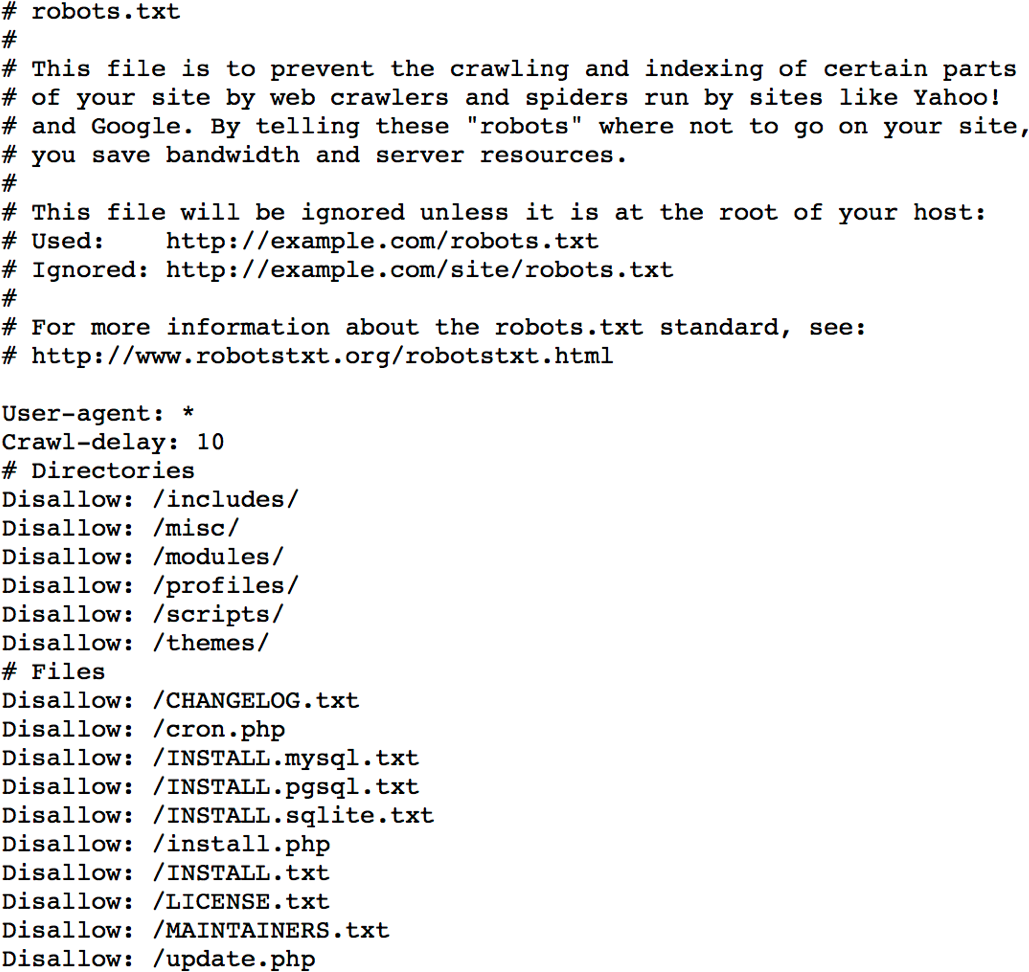
\includegraphics[width=0.40\textwidth]{images/DC/CQADS_robots.png}
\caption[\small \texttt{robots.txt} file for a random webpage]{\small \texttt{robots.txt} file for \newhref{cqads.carleton.ca}{cqads.carleton.ca}.} \hrule\label{fig:robots}
\end{figure}
\afterpage{\FloatBarrier}
\newl Perhaps more importantly, \textbf{be friendly!} Not everything that can be scraped needs to be scraped. Scraping programs should 1) behave ``nicely''; 2) provide useful data, and 3) be efficient, in that order. When in doubt, contact the data provider to see if they will grant access to the databases or files. 
\newpage\noindent Finally, note the importance of following the \textbf{Scraping Do's and Don't's}:
\begin{enumerate}
    \item \textbf{stay identifiable};
    \item \textbf{reduce traffic} -- accept compressed files, check that a file has been changed before accessing it again, retrieve only parts of a file;
    \item \textbf{do not bother server with multiple requests} --  many requests per second can bring smaller server downs, webmasters may block you if your scraper is too greedy (a few requests per second is fine), and
    \item \textbf{write efficient and polite scrapers} -- there is no reason to scrape pages daily or to repeat the same task over and over, select specific resources and leave the rest untouched. 
\end{enumerate}
\paragraph{Web Data Quality} Data quality issues are inescapable. It is not rare for clients to have spent thousands of dollars on data collection (automatic or manual) and to respond to the news that the data is flawed or otherwise unusable with: ``well, it's the best data we have, so find a way to use it.''\par These issues can be side-stepped to some extent if consultants get involved in the project during or prior to the data collection stage, asking questions such as 
\begin{itemize}[noitemsep]
    \item What type of data is best-suited to answer the client's question(s)?
    \item Is the available data of sufficiently high quality to answer the client's question(s)?
    \item Is the available information systematically flawed?
\end{itemize}
Web data can be \textbf{first-hand} information (a tweet or a news article), or \textbf{second-hand} (copied from an offline source or scraped from some online location, which may make it difficult to retrace). \textbf{Cross-referencing} is a standard practice when dealing with secondary data.  \newl Data quality also depends on its \textbf{use(s)} and \textbf{purpose(s)}. For example,
a sample of tweets collected on a random day could be used to analyse the use of a hashtags or the gender-specific use of words, but that dataset might not prove as useful if it had been collected on the day of the 2018 U.S. Presidential Election to predict the election outcomes (due to \textbf{collection bias}).
\newpage\noindent An example might help to illustrate some the pitfalls and challenges. Let's say that a client is interested in finding out what people think of a new potato peeler using a standard telephone survey. 
Such an approach has a number of pitfalls:
\begin{itemize}[noitemsep]
\item\textbf{unrepresentative sample} -- the selected sample might not represent the intended population;
\item\textbf{systematic non-response} -- people who don't like phone surveys might be less (or more) likely to dislike the new potato peeler;  
\item\textbf{coverage error} -- people without a landline can't be reached, say, and 
\item\textbf{measurement error} -- are the survey questions providing suitable info for the problem at hand?
\end{itemize}
Traditional solutions to these problems require the use of survey sampling (more on this later), questionnaire design (see previous section), omnibus surveys, reward systems, audits, etc. These solutions can be \textbf{costly}, \textbf{time-consuming}, and \textbf{ineffective}. \newl \textbf{Proxies} -- indicators that are strongly related to the product's popularity without measuring it directly, could be useful. If \textbf{popularity} is defined as large groups of people preferring a potato peeler over another one, then sales statistics on a commercial website may provide a proxy for popularity. 
\newl Rankings on \texttt{Amazon.ca} (or a similar website) could, in fact, paint a more comprehensive portrait of the potato peeler market than would a traditional survey. It would suffice, then, to build a scraper that is compatible with Amazon's \textbf{application program interface} (API) to gather the appropriate data.\newl Of course, there are potential issues with this approach as well: 
\begin{itemize}[noitemsep]
\item \textbf{representativeness} of the \textbf{listed products} -- Are all potato peelers listed? If not, is it because that website doesn't sell them? Is there some other reason?

\item \textbf{representativeness} of the \textbf{customers} -- Are there specific groups buying/not-buying online products? Are there specific groups buying from specific sites? Are there specific groups leaving/not-leaving reviews? 

\item \textbf{truthfulness} of customers and \textbf{reliability} of reviews -- how can we distinguish between paid (fake) reviews and real reviews?
\end{itemize}
Web scraping is usually well-suited for collecting data on products (such as the aforementioned potato-peeler), but there are numerous questions for which it is substantially more difficult to imagine where data could be found online: what data could you collect online to measure the popularity of a government policy, say? 
\paragraph{Web Technologies 101}
Online data can be found in \textbf{text}, \textbf{tables}, \textbf{lists}, \textbf{links}, and other structures, but the way data is presented in browsers is not necessarily how it is stored in HTML/XML. Furthermore, when web pages are \textbf{dynamic}, there is a ``cost'' associated with automated collection. Consequently, a basic knowledge of the web and web-related techs and documents is crucial. Information is readily available online (see references) and in  \cite{DC_M,DC_MRMN}.\newpage\noindent There are three areas of importance for data collection on the web:
\begin{itemize}[noitemsep]
\item technologies for \textbf{content dissemination} (HTTP, HTML/XML, JSON, plain text, etc.);
\item technologies for \textbf{information extraction} (R, Python XPath, JSon parsers, Beautiful Soup, Selenium, regexps, etc.), and 
\item technologies for \textbf{data storage} (R, Python, SQL, binary formats, plain text formats, etc.).
\end{itemize}
Webpage content itself comes into three main categories: Hypertext Markup Language (HTML; used for web content and code), Cascading Style Sheets (CSS; used for webpage style), and 
JavaScript (js; used for interactivity with the webpage). HTML is, in some sense, the most fundamental; understanding the tree structure of HTML documents, for instance, will go a long way towards helping consultants get full use of the \textbf{scraping toolbox}. 
\paragraph{Scraping Toolbox} Our experience has shown that a number of tools can facilitate the automated data extraction process, including: 
\textit{Developer Tools}, \textit{XPath}, \textit{Beautiful Soup}, \textit{Selenium}, and \textit{regular expressions}. 
\begin{description}
\item[Developer Tools] show the correspondence between the HTML code for a page and the rendered version seen in the browser (see Figure~\ref{fig:erb} for an example). \par Unlike ``View Source'', Developer Tools show the \textit{dynamic} version of the HTML content (i.e. the HTML is shown with any changes made by JavaScript since the page was first received).
\par Inspecting a page's various elements and discovering where they reside in the HTML file is \textbf{crucial} to efficient web scraping: 
\begin{figure}[th!]
\centering
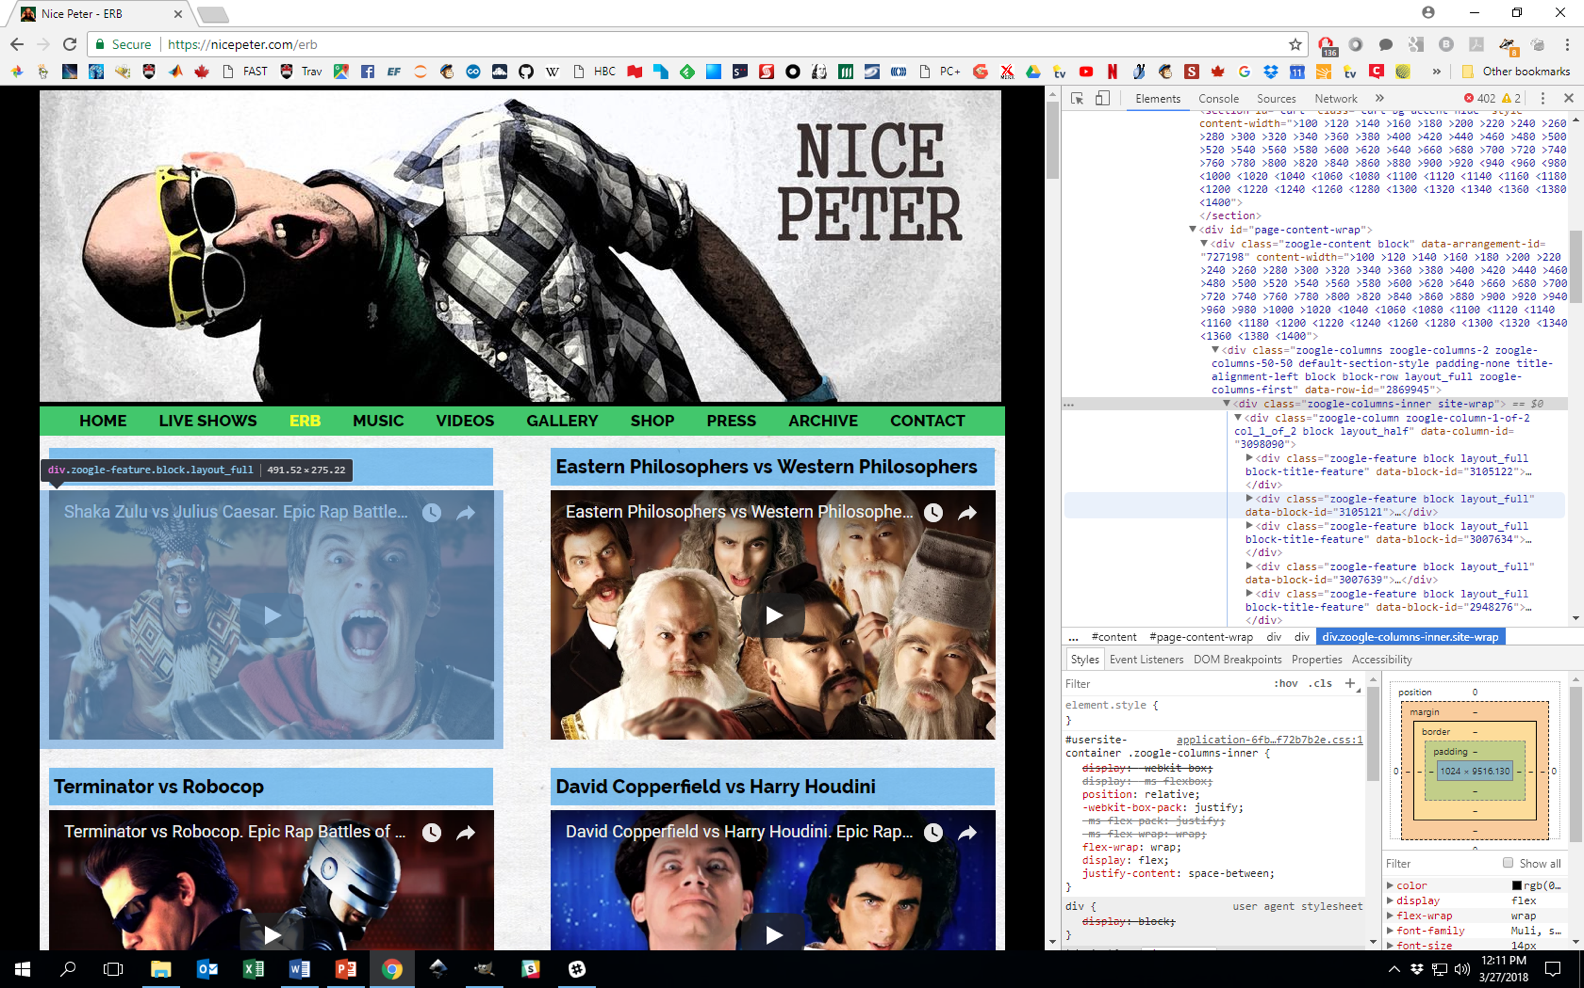
\includegraphics[width=0.95\textwidth]{images/DC/erb.png}
\caption[\small Inspecting a webpage elements using Chrome's \textit{Developer Tools}]{\small Inspecting \newhref{https://nicepeter.com/erb}{nicepeter.com/erb}'s elements using Chrome's \textit{Developer Tools}.} \hrule\label{fig:erb}
\end{figure}
\afterpage{\FloatBarrier}
\begin{itemize}[noitemsep]
\item \textbf{Firefox} -- right click page $\to$ Inspect Element
\item \textbf{Safari} -- Safari $\to$ Preferences $to$ Advanced $\to$ Show Develop Menu in Menu Bar, then  
Develop $\to$ Show Web Inspector
\item \textbf{Chrome} --  right click page $\to$ Inspect
\end{itemize}
\item[XPath] is a query (domain-specific) language which is 
used to select specific pieces of information from marked-up documents such as HTML, XML, or variants such as SVG, RSS. Before this can be done, the information stored in a marked-up document needs to be converted (or \textbf{parsed}) into a format suitable for processing and statistical analysis; this is implemented in the R package XML, for instance. \par The process is simple; it involves 
\begin{enumerate}[noitemsep]
\item specifying the data of interest;
\item locating it in a specific document, and
\item tailoring a query to the document to extract the desired info.
\end{enumerate}
XPath queries require both a \textbf{path} and a \textbf{document} to search; paths consist of hierarchical addressing mechanism (succession of nodes, separated by forward slashes (``/''), while a query takes the form \texttt{xpathSApply(doc,path)}. \par For instance, 
\texttt{xpathSApply(parsed\_doc,``/html/body/div/p/i'')} would find all \texttt{<i>} tags found inside a \texttt{<p>} tag, itself found inside a \texttt{<div>} tag in the \texttt{body} of the \texttt{html} file of \texttt{parsed\_doc}. \par Consult \cite{DC_MRMN} for a substantially heftier introduction. 
\item[Regular Expressions] can be used to achieve the main web scraping objective, which is to extract  relevant information from reams of data. \par Among this mostly unstructured data lurk \textbf{systematic elements}, which can be used to help the automation process, especially if quantitative methods are eventually going to be applied to the scraped data.
\par Systematic structures include numbers, names (countries, etc.), addresses (mailing, e-mailing, URLs, etc.), specific character strings, etc.
\par Regular expressions (regexps) are abstract sequences of strings that match concrete recurring patterns in text; they allow for the systematic extraction of the information components from plain text, HTML, and XML. \par Some examples that illustrate the main concepts are shown in one of the \textit{Jupyter Notebooks} %showcased in Section~\ref{sec:docs}. 
\item[Beautiful Soup] is a Python library that helps extract data out of HTML and XML files. It parses HTML files, even if they're broken. \par Beautiful Soup does not simply convert bad HTML to good X/HTML; it allows a user to fully inspect the (proper) HTML structure it produces, in a programmatical fashion. \par 
When Beautiful Soup has finished its work on an HTML file, the resulting \textit{soup} is an API for \textbf{traversing}, \textbf{searching}, and \textbf{reading} the document's elements. In essence, it provides \textbf{idiomatic} ways of navigating, searching, and modifying the parse tree of the HTML file, which can save a fair amount of time.
\par For instance, \texttt{soup.find\_all('a')} would find and output all \texttt{<a ...> ... </a>} tag pairs (with attributes and content) in the \texttt{soup}, whereas \begin{quote}\texttt{for link in soup.find\_all('a'):}\newline \texttt{\ \ \ print(link.get('href')}
\end{quote} would output the URLs found in the same tag pairs. \par The Beautiful Soup documentation is quite explicit \cite{DC_BS}. 
\item[Selenium] is a Python tool used to automate web browser interactions.  It is used primarily for testing purposes, but it has data extraction uses as well. 
\par Mainly, it allows the user to open a browser and to act as a human being would:
\begin{itemize}[noitemsep]
    \item clicking buttons;
\item entering information in forms;
\item searching for specific information on a page, etc.
\end{itemize}
Selenium requires a driver to interface with the chosen browser. Firefox, for example, uses \texttt{geckodriver}.

Other supported browsers have their own drivers (see \cite{DC_S_C,DC_S_E,DC_S_F,DC_S_S}).

Selenium automatically controls a complete browser, including rendering the web documents and running JavaScript. This is useful for pages with a lot of dynamic content that isn't in the base HTML.

Selenium can program actions like ``click on this button'', or ``type this text'', to provide access to the dynamic HTML of the current state of the page, not unlike what happens in  \textit{Developer Tools} (but now the process can be fully automated).

More information can be found in \cite{DC_S,DC_S2}.
\end{description}
\begin{center}
    \rule{0.5\textwidth}{.4pt}
\end{center}
Let us end this section by providing a short summary of the \textbf{automated data collection decision process} \cite{DC_MRMN,DC_M}, as seen by  quantitative consultants. 
\begin{enumerate}
    \item \textbf{Know exactly what kind of information the client needs}, either \textbf{specific} (e.g. GDP of all OECD countries for last 10 years, sales of top 10 tea brands in 2017, etc.) or \textbf{vague} (people's opinion on tea brand $X$, etc.)
\item \textbf{Find out if there are any web data sources that could provide direct or indirect information on the client's problem.} That is easier to achieve for specific facts (a tea store's webpage will provide information about teas that are currently in demand) than it is for vague facts. Tweets and social media platforms may contain opinion trends; commercial platforms can provide information on product satisfaction.
\item \textbf{Develop a theory of the data generation process when looking into potential data sources.} When was the data generated? When was it uploaded to the Web? Who uploaded the data? Are there any potential areas that are not covered, consistent, or accurate? How often is the data updated?
\item \textbf{Balance the advantages and disadvantages of potential data sources.} Validate the quality of data used -- are there other independent sources that provide similar information against which to crosscheck? Can original source of secondary data be identified?
\item \textbf{Make a data collection decision}. Choose the data sources that seem most suitable, and document reasons for this decision. Collect data from several sources to validate the final choice. 
\end{enumerate}
\subsubsection{Statistical Survey Sampling} 
\begin{tcolorbox}[title=You Can't Say It's Not True]
%Figures often beguile me, particularly when I have the arranging of them myself; in which case the remark attributed to Disraeli would often apply with justice and force: 'There are three kinds of lies: lies, damned lies, and statistics.' 
The latest survey shows that 3 out of 4 people make up 75\% of the world's population.\\[-0.6cm]
\begin{flushright}
%-- Mark Twain, \textit{Chapters of My Autobiography}, 1906
-- David Letterman (attributed)
\end{flushright}
\end{tcolorbox}
\noindent
While the \textit{World Wide Web} does contain troves of data, web scraping does not address the question of data validity: will the extracted data be \textbf{useful} as an analytical component? Will it  suffice to provide the quantitative answers that the client is seeking? 
\newl A \textbf{survey} (a fair amount of information for this section is taken from \cite{DC_F,DC_SC}) is any activity that collects information about characteristics of interest:
\begin{itemize}[noitemsep] 
\item in an \textbf{organized} and \textbf{methodical} manner;
\item from some or all \textbf{units} of a population;
\item using \textbf{well-defined} concepts, methods, and procedures, and
\item compiles such information into a \textbf{meaningful} summary form. 
\end{itemize}
A \textbf{census} is a survey where information is collected from all units of a population, whereas a \textbf{sample survey} uses only a fraction of the units. 
\begin{figure}[t!]
\centering
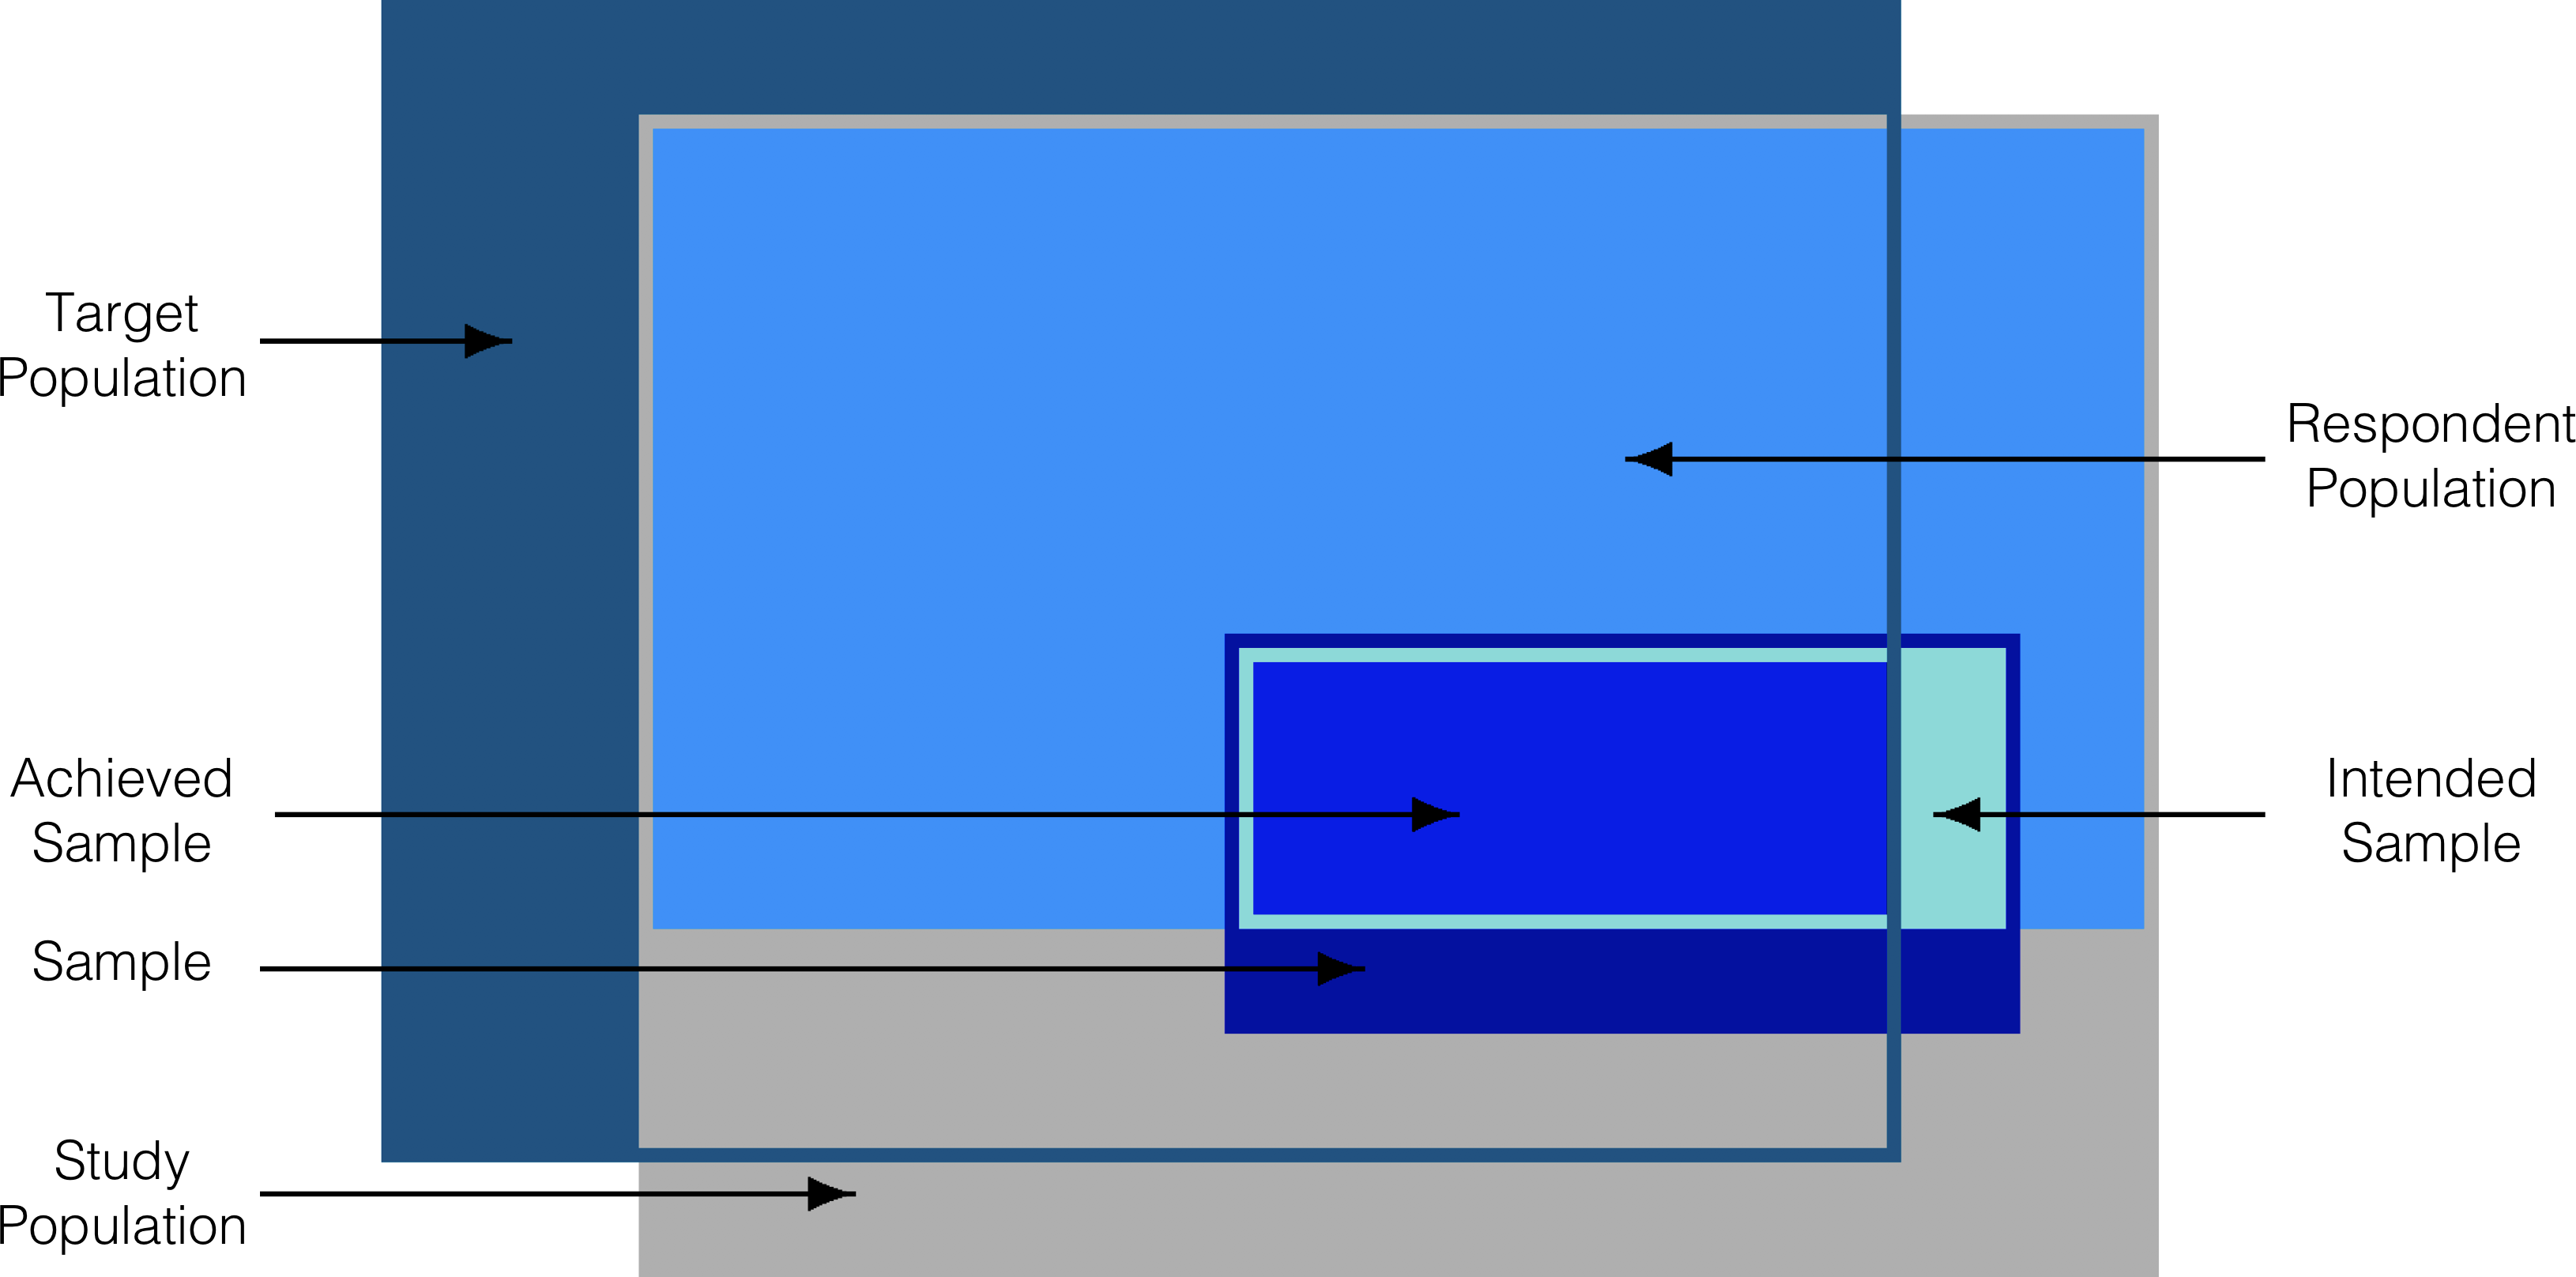
\includegraphics[width=0.95\textwidth]{images/DC/SamplingDesign.png}
\caption[\small The sampling model]{\small Various populations and samples in the sampling model.} \hrule\label{fig:sammod}
\end{figure}
\afterpage{\FloatBarrier}
\paragraph{Sampling Model}
When survey sampling is done properly, we may be able to use various statistical methods to make inferences about the \textbf{target population} by sampling a (comparatively) small number of units in the \textbf{study population}. The relationship between the various populations (\textbf{target}, \textbf{study}, \textbf{respondent}) and samples (\textbf{sample}, \textbf{intended}, \textbf{achieved}) is illustrated in Figure~\ref{fig:sammod}. 
\paragraph{Deciding Factors} In some instances, information about the \textbf{entire} population is required in order to solve the client's problem, whereas in others it is not necessary.  How does one determine which type of survey must be conducted to collect data? The answer depends on multiple factors: 
\begin{itemize}[noitemsep]
    \item the type of question that needs to be answered;
\item the required precision;
\item the cost of surveying a unit;
\item the time required to survey a unit; \item size of the population under investigation, and 
\item the prevalence of the attributes of interest.
\end{itemize}
Once a choice has been made, each survey typically follows the same \textbf{general steps}:
\begin{enumerate}[noitemsep]
    \item statement of objective
    \item selection of survey frame
    \item sampling design
    \item questionnaire design
    \item data collection
    \item data capture and coding
    \item data processing and imputation
    \item estimation
    \item data analysis
    \item dissemination
    \item documentation
\end{enumerate}
The process is not always linear, in that preliminary planning and data collection may guide the implementation (selection of a frame and of a sampling design, questionnaire design), but there is a definite movement from objective to dissemination.   
\paragraph{Survey Frames} The \textbf{frame} provides the means of \textbf{identifying} and \textbf{contacting} the units of the study population. It is generally costly to create and to maintain (in fact, there are organisations and companies that specialise in building and/or selling such frames). Useful frames contain: 
\begin{itemize}[noitemsep]
\item identification data, 
\item contact data, 
\item classification data,
\item maintenance data, and 
\item linkage data.
\end{itemize} \newpage\noindent The ideal frame must minimize the risk of \textbf{undercoverage} or \textbf{overcoverage}, as well as the number of \textbf{duplications} and \textbf{misclassifications} (although some issues that arise can be fixed at the data processing stage).\par Unless the selected frame is \textbf{relevant} (which is to say, it corresponds, and permits accessibility to, the target population), \textbf{accurate} (the information it contains is valid), \textbf{timely} (it is up-to-date), and \textbf{competitively priced}, the statistical sampling approach is contraindicated. 
\paragraph{Survey Error} 
One of the strengths of statistical sampling is in its ability to provide estimates of various quantities of interest in the target population, and to provide some control over the  \textbf{total error} (TE) of the estimates. The TE of an estimate is the amount by which it differs from the true value for the target population:
\begin{align*} 
\TE  & =  \ME  +  \SE +  \NE +  \CE, \end{align*}
where the 
\begin{itemize}[noitemsep]
\item \textbf{coverage error} is due to differences in the study and target populations; 
\item \textbf{non-response error} is due to differences in the respondent and study populations;
\item \textbf{sampling error} is due to differences in the achieved sample and the respondent population; 
\item \textbf{measurement error} is due to true value in the achieved sample not assessed correctly.
\end{itemize}
If we let 
\begin{itemize}[noitemsep]
\item $\overline{x}$ be the computed attribute value in the achieved sample; 
\item $\overline{x}_{\mathrm{true}}$ be the true attribute value in the achieved sample under perfect measurement;
\item $x_{\mathrm{resp}}$ be the attribute value in the respondent population;
\item $x_{\mathrm{study}}$ be the attribute value in the study population, and 
\item $x_{\mathrm{tar}}$ be the attribute value in the target population,
\end{itemize}
then 
$\TE  = \overline{x} - x_{\mathrm{tar}} =  (\overline{x} - \overline{x}_{\mathrm{true}}) + (\overline{x}_{\mathrm{true}}-x_{\mathrm{resp}}) + (x_{\mathrm{resp}}-x_{\mathrm{study}}) + (x_{\mathrm{study}}-x_{\mathrm{tar}}).$\newl In an ideal scenario, $\TE=0$. In practice, there are two main contributions to $\TE$: \textbf{sampling errors} (which we will discuss shortly) and \textbf{nonsampling errors}, which include every contribution to survey error which is not due to the choice of sampling scheme. The latter can be controlled, to some extent: 
\begin{itemize}[noitemsep]
\item \textbf{coverage error} can be minimized by selecting a high quality, up-to-date survey frame;
\item \textbf{non-response error} can be minimized by careful choice of the data collection mode and questionnaire design, and by using ``call-backs'' and ``follow-ups'';
\item \textbf{measurement error} can be minimized by careful questionnaire design, pre-testing of the measurement apparatus, and cross-validation of answers.  
\end{itemize}
In practice, these suggestions are perhaps less useful than one could hope in modern times: survey frames based on landline telephones are quickly becoming irrelevant in light of an increasingly large and younger population who eschew such phones, for instance, while response rates for surveys that are not mandated by law are  surprisingly low. This explains, in part, the impetus towards automated data collection and the use of \textbf{non-probabilistic sampling} methods.     
\paragraph{Modes of Data Collection}
How is data traditionally captured, then? There are \textbf{paper-based} approaches, \textbf{computer-assisted} approaches, and a suite of other modes.  
\begin{itemize}[noitemsep]
\item \textbf{Self-administered questionnaires} are used when the survey requires detailed information to allow the units to consult personal records (which reduces measurement errors), they are useful to measure responses to sensitive issues as they provide an extra layer of privacy, and are typically not as costly as other collection modes, but they tend to be associated with high non-response rate since there is less pressure to respond. 
\item \textbf{Interviewer-assisted questionnaires} use well-trained interviewers to  increase the response rate and overall quality of the data.\par  Face-to-face \textbf{personal interviews} achieve the highest response rates, but they are costly (both in training and in salaries). Furthermore, the interviewer may be required to visit any selected respondents many times before contact is established. \par \textbf{Telephone interviews}, on the other hand produce ``reasonable'' response rates at a reasonable cost and they are safer for the interviewers, but they are limited in length due to respondent phone fatigue. With random dialing, 4-6 minutes of the interviewer's time is spent in out-of-scope numbers for each completed interview.
\item \textbf{computer-assisted interviews} combine data collection and data capture, which saves valuable time, but the drawback is that not every sampling unit may have access to a computer/data recorder (although this is becomine less prevalent). \par All paper-based modes have a computer-assisted equivalent: \textbf{computer-assisted self-interview} (CASI), \textbf{computer-assisted interview} (CAI),  \textbf{computer-assisted telephone interview} (CATI), and 
\textbf{Computer-assisted personal interview} (CAPI).
\item Unobtrusive direct observation
\item Diaries to be filled (paper or electronic)
\item Omnibus surveys
\item Email, Internet, and social media (see Section~\ref{sec:adc})
\end{itemize}
\paragraph{Non-Probabilistic Sampling}
There exists a number of methods to select sampling units from the target population that use subjective, non-random approaches (NPS). These methods tend to be \textbf{quick}, \textbf{relatively inexpensive} and \textbf{convenient} in that a survey frame is not needed. NPS methods are ideal for \textbf{exploratory analysis} and \textbf{survey development}. \newl Unfortunately, they are sometimes used \textbf{instead} of probabilistic sampling designs, which is problematic; the associated selection bias makes NPS methods \textbf{unsound} when it comes to \textbf{inferences}, as they cannot be used to provide \textbf{reliable estimates of the sampling error} (the only component of $\TE$ on which the analysts has direct control). Automated data collection often fall squarely in the NPS camp, for instance. While we can still analyse data collected with a NPS approach, we \textbf{may not generalise the results} to the target  population (except in rare, census-like situations). \newl
NPS methods include
\begin{itemize}[noitemsep]
\item \textbf{Haphazard} sampling, also known as `man on the street' sampling; it assumes that the population is homogeneous, but the selection remains subject to interviewer biases and the availability of units;
\item \textbf{Volunteer} sampling in which the  respondents are self-selected; there is a large selection bias since the silent majority does not usually volunteer; this method is often imposed upon analysts due to ethical considerations; it is also used for focus groups or qualitative testing;
\item \textbf{Judgement} sampling is based on the analysts' ideas of the target population composition
 and behaviour (sometimes using a prior study); the units are selected by population experts, but inaccurate preconceptions can introduce large biases in the study;
\item \textbf{Quota} sampling is very common (and is used in exit polling to this day in spite of the infamous ``Dewey Defeats Truman'' debacle of 1948 \cite{DC_DDT}); sampling continues until a
 specific number of units have been selected for various sub-populations; it is preferable to
 other NPS methods because of inclusion of sub-populations, but it ignores non-response bias;
\item \textbf{Modified} sampling starts out using probability sampling (more on this later), but turns to quota sampling in its last stage, in part as a reaction to high non-response rates;
\item \textbf{Snowball} sampling asks sampled units to recruit other units among their acquaintances; this NPS approach may help locate hidden populations, but it biased in favour of units with larger social circles and units that are charming enough to convince their acquaintances to participate. 
\end{itemize}
\begin{center}
    \rule{0.5\textwidth}{.4pt}
\end{center}
There are contexts where NPS methods might fit a client's need (and that remains their decision to make, ultimately), but the consultant MUST still inform the client of the drawbacks, and present some  probabilistic alternatives.  
\paragraph{Probabilistic Sampling}
The inability to make sound inferences in NPS contexts is a monumental strike against their use. While probabilistic sample designs are usually \textbf{more difficult and expensive} to set-up (due to the need for a quality survey frame), and take \textbf{longer} to complete, they provide \textbf{reliable estimates} for the attribute of interest and the sampling error, paving the way for  small samples being used to draw inferences about  larger target populations (in theory, at least; the non-sampling error components can still affect results and generalisation). \newl We shall take a deeper look at traditional probability sample designs such as \textbf{simple random}, \textbf{stratified random}, and \textbf{systematic},   -- \textbf{cluster}, \textbf{probability proportional to size}, \textbf{replicated}, \textbf{multi-stage} and \textbf{multi-phase} variants also exist (see \cite{DC_F,DC_SC} for details).\newl
Let us start with some basic mathematical concepts. Consider a finite population $\mathcal{U}=\{u_1,\ldots,u_N\}$. The \textbf{mean} and \textbf{variance} of the population are given by 
$$\mu=\frac{1}{N}\sum_{j=1}^Nu_j\quad\mbox{and}\quad \sigma^2=\frac{1}{N}\sum_{j=1}^N(u_j-\mu)^2, \quad\mbox{respectively.}$$ If $\mathcal{Y}=\{y_1,\ldots,y_n\}$ is a sample of $\mathcal{U}$, the \textbf{sample mean} and \textbf{sample variance} (also known as the \textbf{empirical mean} and \textbf{empirical variance}) are given by 
$$\overline{y}=\frac{1}{n}\sum_{i=1}^ny_i\quad\mbox{and}\quad S^2=\frac{1}{n-1}\sum_{i=1}^n(y_i-\overline{y})^2, \quad\mbox{respectively.}$$ Let $X_1,\ldots,X_n$ be random variables, $b_1,\ldots,b_n\in \mathbb{R}$, and $\GE$, $\GV$, and $\GC$ be the \textbf{expectation}, \textbf{variance} and \textbf{covariance} operators, respectively. Recall that 
\begin{align*}
    \GE \left(\sum_{i=1}^nb_iX_i\right) &=\sum_{i=1}^nb_i\GE(X_i) \\
    \GV\left(\sum_{i=1}^nb_iX_i\right)&=\sum_{i=1}^n b_i^2\GV(X_i)+\sum_{1\leq i\neq j}^nb_ib_j\GC(X_i,X_j) \\
\GC(X_i,X_j)&=\GE(X_iX_j)-\GE(X_i)\GE(X_j)\\
\GV(X_i)&=\GC(X_i,X_i)=\GE\left(X_i^2\right)-\GE^2(X_i).
\end{align*}
The \textbf{bias} in an error component is the average of that error component if the survey is repeated many times independently under the same conditions. The \textbf{variability} in an error component is the extent to which that component would vary about its average value in the ideal scenario described above. The \textbf{mean square error} of an error component is a measure of the size of the error component:
\begin{align*}
\MSE(\hat{\beta})&=\GE\left((\hat{\beta}-\beta)^2\right)=\GE\left((\hat{\beta}-\GE(\hat{\beta})+\GE(\hat{\beta})-\beta)^2\right)\\&=\GV(\hat{\beta})+\left(\GE(\hat{\beta})-\beta\right)^2=\GV(\hat{\beta})+\Bias^2(\hat{\beta}) \end{align*}
where $\hat{\beta}$ is an estimate of $\beta$. Incidentally, the unusual denominator in the sample variance insures that it is an unbiased estimator of the population variance.\newl Finally, if the estimate is unbiased, then an approximate \textbf{95\% confidence interval} (95\% CI) for $\beta$ is given by $$\hat{\beta}\pm 2\sqrt{\hat{\GV}(\hat{\beta})},$$ where $\hat{\GV}(\hat{\beta})$ is a sampling design-specific estimate of $\GV(\hat{\beta})$.
\begin{center}
    \rule{0.5\textwidth}{.4pt}
\end{center}
In what follows, we discuss a number of sampling designs and present some of their advantages and disadvantages. We also show how to compute estimates for various population attributes (mean, total, proportion, ratio, difference, regression) and how to estimate the corresponding 95\% CI. Finally, we briefly discuss how to compute sample sizes for a given \textbf{error bound} (an upper limit on the radius of the desired 95\% CI), and how to determine the \textbf{sample allocation} (how many units to be sampled in various sub-population groups), for designs where it is appropriate to do so. \newl 
In all instances, the target population consists of $N$ measurements/units, $\mathcal{U}=\{u_1,\ldots,u_N\}$, and the true population mean, population variance, population total, and population proportion for the variable of interest are $\mu$, $\sigma^2$, $\tau$, and $p$, respectively. The sample is a subset of the target population, $\mathcal{Y}=\{y_1,\ldots,y_n\}\subseteq \mathcal{U}$ from which we estimate the respective population attributes \textit{via} $\overline{y}$, $s^2$, $\hat{\tau}$, and $\hat{p}$. \par For a given characteristic, we define $\delta_i$ as $1$ or $0$ depending on whether the corresponding sample unit $y_i$ possesses the characteristic in question or not. Lastly, we set the error bound to $B=2\sqrt{\hat{V}}>0$.\newpage\noindent 
In \textbf{Simple Random Sampling} ($\SRS$), $n$ units are selected randomly from the survey frame, as in Figure~\ref{fig:SRS}. \begin{figure}[t]
\centering
\begin{subfigure}[b]{0.30\textwidth}
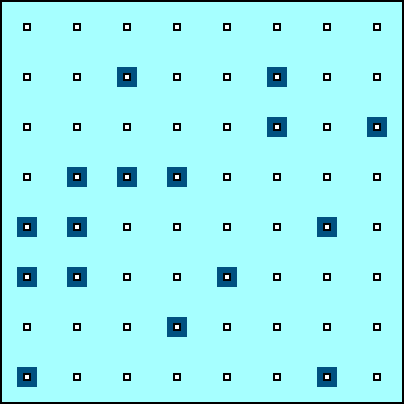
\includegraphics[width=\textwidth]{images/DC/Sampling_SRS.png}
\caption{\small Simple Random} 
\label{fig:SRS}
\end{subfigure}\quad
\begin{subfigure}[b]{0.30\textwidth}
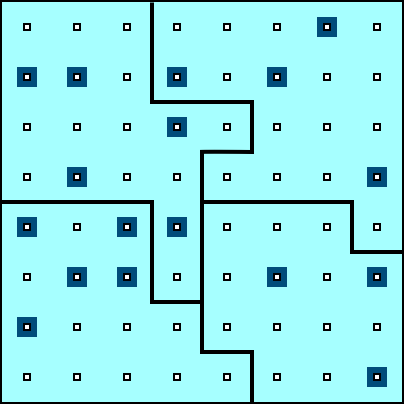
\includegraphics[width=\textwidth]{images/DC/Sampling_StS.png}
\caption{\small Stratified} 
\label{fig:StS}
\end{subfigure}\quad
\begin{subfigure}[b]{0.30\textwidth}
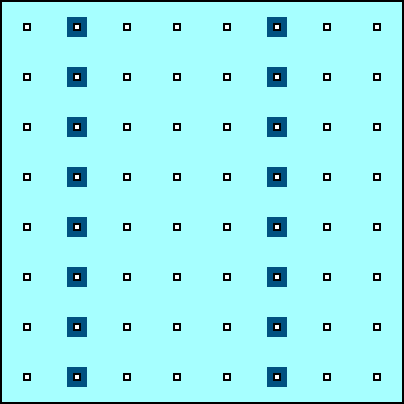
\includegraphics[width=\textwidth]{images/DC/Sampling_SyS.png}
\caption{\small Systematic} 
\label{fig:SyS}
\end{subfigure}
\begin{subfigure}[b]{0.30\textwidth}
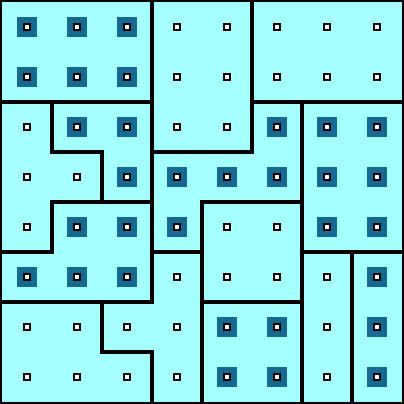
\includegraphics[width=\textwidth]{images/DC/Sampling_ClS.png}
\caption{\small Cluster} 
\label{fig:ClS}
\end{subfigure}\quad
\begin{subfigure}[b]{0.30\textwidth}
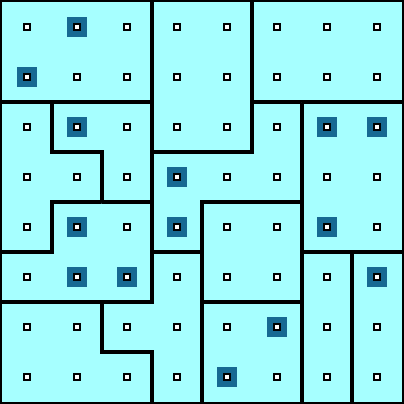
\includegraphics[width=\textwidth]{images/DC/Sampling_MSS.png}
\caption{\small Multi-Stage} 
\label{fig:MPS}
\end{subfigure}\quad
\begin{subfigure}[b]{0.30\textwidth}
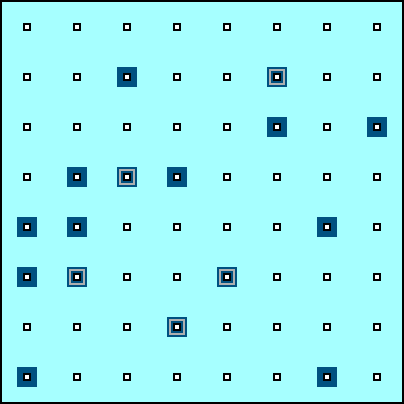
\includegraphics[width=\textwidth]{images/DC/Sampling_MPS.png}
\caption{\small Multi-Phase} 
\label{fig:MSS}
\end{subfigure}
\caption[\small Schematics of sampling designs]{\small Schematics of sampling designs.}
\hrule\label{fig:designs}
\end{figure}
\afterpage{\FloatBarrier}
It is by far the easiest sampling design to implement, and estimates for the resulting sampling errors are well known and easy to compute, which leads to $\SRS$ often being used at a later stage in the sampling process. 
Another advantage is that $\SRS$ does not require auxiliary information, which can be useful with more economical survey frames. \newl This can backfire however, as $\SRS$ makes no use of such information even when it is available. There is also no guarantee that the sample will be representative of the population. Note as well that $\SRS$ may be costly if the sample is widely spread out, geographically.\newl 
The $\SRS$ estimators are 
$$\overline{y}=\frac{1}{n}\sum_{i=1}^n y_i, \quad \hat{\tau}=N\overline{y}, \quad\mbox{and}\quad \hat{p}=\frac{1}{n}\sum_{i=1}^n \delta_i$$ with respective variances
$$\GV(\overline{y})=\frac{\sigma^2}{n}\left(\frac{N-n}{N-1}\right),\quad \GV(\hat{\tau})=N^2\cdot\frac{\sigma^2}{n}\left(\frac{N-n}{N-1}\right),\quad\mbox{and}\quad \GV(\hat{p})=\frac{p(1-p)}{n}\left(\frac{N-n}{N-1}\right).$$
\newpage\noindent The 95\% CI is approximated by substituting the true variance $\sigma^2$ by the unbiased estimator $\frac{n-1}{n}s^2$: $$\hat{\GV}(\overline{y})=\frac{s^2}{n}\left(1-\frac{n}{N}\right), \quad
\hat{\GV}(\hat{\tau})=N^2\cdot\frac{s^2}{n}\left(1-\frac{n}{N}\right), \quad\mbox{and}\quad 
\hat{\GV}(\hat{p})=\frac{\hat{p}(1-\hat{p})}{n-1}\left(1-\frac{n}{N}\right).$$
Finally, the sample size required to achieve an upper error bound $B$ are $$n_{\overline{y}}=\frac{4N\sigma^2}{(N-1)B^2+4\sigma^2},\quad n_{\hat{\tau}}=\frac{4N^3\sigma^2}{(N-1)B^2+4N^2\sigma^2},\quad\mbox{and}\quad n_{\hat{p}}=\frac{4Np(1-p)}{(N-1)B^2+4p(1-p)},$$ where $\sigma^2$ and $p$ have been previously estimated (perhaps as part of a prior survey). \newl 
In \textbf{Stratified Random Sampling} ($\StS$), $n=n_1+\cdots+n_k$ units are selected randomly from the survey frame by first establishing $k$ natural strata (such as provinces, or age groups), and selecting $n_j$ units from the $N_j$ units in stratum $j$, with $\overline{y}_j$ and $\hat{p}_j$ the $\SRS$ estimators in stratum $j$, $j=1,\ldots, k$. An illustration is provided in Figure~\ref{fig:StS}. \newl $\StS$ may produce a smaller bound on the error of estimation than would be produced by a $\SRS$ of the same size, particularly if measurements within a strata are homogeneous, and it may be less expensive to implement if the elements are stratified into convenient groupings. Another added benefits is that it may provide parameter estimates for sub-populations that coincide with the strata (see Section~\ref{sec:DC_CS} for an application). There are no major disadvantage to this sample design, except for the fact that there might not be natural ways to stratify the frame (in the sense that each stratum might not be homogeneous in its units), in which case $\StS$ is roughly equivalent to $\SRS$. \newl The $\StS$ estimators are 
$$\overline{y}_{\textrm{st}}=\sum_{j=1}^k \frac{N_j}{N}\overline{y}_j, \quad \hat{\tau}_{\textrm{st}}=N\overline{y}_{\textrm{st}}, \quad\mbox{and}\quad \hat{p}_{\textrm{st}}=\sum_{j=1}^k \frac{N_j}{N}\hat{p}_j,$$ with approximate variances given by 
$$\hat{\GV}(\overline{y}_{\textrm{st}})=\frac{1}{N^2}\sum_{j=1}^kN_i^2\hat{\GV}\left(\overline{y}_j\right),\quad \hat{\GV}(\hat{\tau}_{\textrm{st}})=N^2\hat{\GV}(\overline{y}_{\textrm{st}}),\quad\mbox{and}\quad \hat{\GV}(\hat{p}_{\textrm{st}})=\frac{1}{N^2}\sum_{j=1}^kN_i^2\hat{\GV}\left(\overline{p}_j\right).$$
In the $\StS$ design, the sample determination question is two-fold: what size $n$ should the sample have, and how should they be allocated to each stratum ($n_j$, $j=1,\ldots,k$). \par We can select $n$ based on \textbf{cost} considerations or on error bound considerations. Let $c_0$ be the fixed survey operation costs (\textbf{overhead}), $c_j$ be the \textbf{cost per response} in  stratum $j$ (which may need to include the cost of trying to reach non-respondents), and $C$ be the \textbf{total cost} of conducting the survey. The sample size $n$ that minimises  $\hat{\GV}(\overline{y}_{\mbox{st}})$ subject to   $C=c_0+\sum_{j=1}^kc_jn_j$ and $n=\sum_{j=1}^kn_j$ is $$n_{\textrm{st},C}=(C-c_0)\frac{\sum_{j=1}^k \frac{N_j\sigma_j}{\sqrt{c_j}}}{\sum_{j=1}^k N_j\sigma_j\sqrt{c_j}}.$$ In the \textbf{general optimum allocation scheme}, the sampling weights (by strata) are $$w_j=\frac{n_j}{n}=\frac{N_j\sigma_jc_{j}^{-1/2}}{\sum_{\ell=1}^kN_{\ell}\sigma_{\ell}c_{\ell}^{-1/2}}.$$ 
In the \textbf{Neyman allocation scheme}, we assume that the cost per response is identical in each stratum, whence 
$$w_{j,N}=\frac{n_j}{n}=\frac{N_j\sigma_j}{\sum_{\ell=1}^kN_{\ell}\sigma_{\ell}},$$ while in the \textbf{proportional allocation scheme} we further assume that $\sigma_j=\sigma$ for all $j$, so that $$w_{j,P}=\frac{n_j}{n}=\frac{N_j}{N}.$$ Other allocation schemes are also sometimes selected, such as the \textbf{square root proportional scheme} which fixes $$w_{j,S}=\frac{N_j^{1/2}}{\sum_{\ell=1}^kN_{\ell}^{1/2}}$$ in order to insure that smaller strata (e.g. provinces with smaller populations, say) are allocated enough observations to produce sub-population estimates. \newl Note that while budgetary considerations need to be considered in practice, the preceding approach does not allow prescribed error bounds, which could prove problematic. The sample size required to achieve an upper error bound $B$ are\small $$n_{\textrm{st},\overline{y}}=\frac{4\sum_{j=1}^k\frac{N_j\sigma_j^2}{w_j}}{N^2B^2+4\sum_{j=1}^kN_j\sigma_j^2},\quad n_{\textrm{st},\hat{\tau}}=\frac{4N^2\sum_{j=1}^k\frac{N_j\sigma_j^2}{w_j}}{N^2B^2+4\sum_{j=1}^kN_j\sigma_j^2},\quad\mbox{and}\quad n_{\textrm{st},\hat{p}}=\frac{4\sum_{j=1}^k\frac{N_jp_j(1-p_j)}{w_j}}{N^2B^2+4\sum_{j=1}^kN_jp_j(1-p_j)},$$ \normalsize where $\sigma_j^2$ and $p_j$ have been previously estimated, and a specific allocation scheme  $\{w_j\}$ has already been selected. 
In \textbf{Systematic Sampling} ($\SyS$), $n$ units are selected randomly from the survey frame by first (randomly) selecting a unit $y_1$ among the first $k=\lfloor\frac{N}{n}\rfloor$ units in the frame and s systematically adding every subsequent $k^{\textrm{th}}$ unit to the sample. An illustration is provided in Figure~\ref{fig:SyS}. \newl $\SyS$ is typically appropriate when the frame is already \textbf{sorted} along the characteristic of interest in which case it provides greater information by unit cost than $\SRS$. It is simpler to implement than $\SRS$ since only one random number is required, and like $\SRS$, it does not require auxiliary frame information. Depending on the sample size and on how the frame is sorted, $\SyS$ can produce a sample that is more widely spread (and thus perhaps more representative) than $\SRS$, which may help eliminate other sources of bias.\par On the other hand, it can introduce bias when the pattern used for the systematic sample coincides with a pattern in the population, and it makes no use of auxiliary frame information even if such information exists. Furthermore, any advantage in precision over $\SRS$ disappears if the frame is randomly ordered. Embarrassingly, $\SyS$ may lead to a variable sample size if $n$ does not evenly divide $N$; perhaps more importantly, $\SyS$ does not allow for an unbiased estimator of the sampling variance.\newl For all practical purposes, $\SyS$ behaves like $\SRS$ for a random population. In that case, the $\SRS$ variance  formula may provide a decent approximation. 
\par If the frame is \textbf{ordered} along the characteristic of interest, each $\SyS$ sample will contain some of the smaller values as well as some of the larger values, which would not necessarily be the case in a general $\SRS$ sample. This implies that the  $\SyS$ estimators will have smaller variances than the corresponding $\SRS$ estimators, so that the use of the $\SRS$ variance formula produces an overestimate of the true sampling error in that case. \par In a similar vein, a population is \textbf{periodic} if the frame is \textbf{periodic}  along the characteristic of interest, a $\SyS$ sample that hits both the peaks and valleys of a cyclical trend will bring the method more in line with $\SRS$ and allow the use of the $\SRS$ variance formula as a reasonable approximation. To avoid the problem of underestimating the variation, consider changing the random starting point several times.\newl 
If $n$ divides $N$ evenly, then systematic sampling can be viewed as grouping the population into $k=N/n$ strata, and selecting one unit from each stratum. The difference between $\SyS$ and $\StS$ is that only the first unit is picked randomly in $\SyS$ -- all other samples are automatically selected based on the position of the first choice. \par One can also view $\SyS$ as a one-stage cluster sampling (see the next sub-section), where a primary sampling unit is defined as one of the $k=N/n$ possible systematic samples. An $\SRS$ of one unit can then be drawn from these $k$ primary sampling units. The $\SyS$ sample will consist of all of the items in the selected primary sample.
\newl The $\SyS$ estimators are computed exactly as the corresponding $\SRS$ estimators; their variances are given by  
$$\GV(\overline{y}_{\textrm{sys}})=\frac{\sigma^2}{n}[1+(n-1)\rho],\quad  \GV(\hat{\tau}_{\textrm{sys}})=N^2\GV(\overline{y}_{\textrm{sys}}),\quad\mbox{and}\quad \GV(\hat{p}_{\textrm{sys}})=\frac{p(1-p)}{n}[1+(n-1)\rho],$$ where $\rho$ is the \textbf{intra-cluster correlation} (which is typically impossible to compute exactly). 
\begin{center}
    \rule{0.5\textwidth}{.4pt}
\end{center}
Other sampling schemes tend to be substantially more complicated (in the sense that the estimators and variance estimates are harder to derive), but the conceptual ideas behind those sampling schemes are still pretty straightforward; if required, in-depth details can be found in \cite{DC_SC}.
\newl \textbf{Cluster Sampling}
 ($\ClS$), for instance is typically used when the data collection cost increases with the ``distance'' separating the element. The population is separated in clusters, and an $\SRS$ of clusters is selected -- all units within a selected clusters are retained in the sample (see Figure~\ref{fig:ClS} for an illustration). As an example, to sample individuals in the population without a population frame (which might be hard to come by), it might be easier to obtain a dwelling frame and to start by sampling dwellings (which are the population \textbf{clusters}), and then to select all individuals in the sampled dwellings. $\ClS$ surveys are usually less expensive and less time-consuming to conduct than $\SRS$, and they can be used to show ``regional'' variations, but they will be wasteful if the cluster sizes are too large, and biased if only a few clusters are sampled.  
 
\subsubsection{Case Study: Canada Vehicle Use Study}
\label{sec:DC_CS}
The \textbf{Canadian Vehicle Survey} (CVS) was sponsored by  \textit{Transport Canada} (TC) and \textit{Natural Resources Canada} between 1999 and 2009. The quarterly survey employed a \textbf{two-stage sample design}: a sample of vehicles was selected and then a period of travel within the quarter was selected for each vehicle. \newl 
Vehicles were grouped into three categories: \textit{light vehicles} (passenger cars and light trucks/vans) and two types of \textit{heavy vehicles}, based on the gross vehicle weight. A \textbf{paper questionnaire} was then mailed out to the owners of the selected vehicles, requesting that they record the \textit{number of trips}, \textit{distance driven}, and \textit{fuel consumption} during the observation period.\par
The CVS was hampered by low participant response rates  over its duration ($\approx 20\%$), caused in large part by the \textbf{burdensome paper collection} methods. The quality of the estimates was also weakened by \textbf{significant errors} in the way in which the on-road vehicle fleet was classified due to mistakes in the \textit{Vehicle Identification Number} (VIN) decoding code.
\newl  As a result, TC decided to conduct a pilot \textbf{Canadian Vehicle Use Study} (CVUS) to validate (or invalidate) the CVS methodology and results. Improvements included 
\begin{itemize}[noitemsep]
\item  the use of \textbf{electronic data loggers} to reduce reporting burden; 
\item the introduction of a more \textbf{robust} VIN decoder to increase the accuracy of the in-scope fleet, and 
\item a \textbf{modified sampling design} that incorporated additional strata to enhance the ability to carry out more detailed analyses of motor vehicle use.
\end{itemize}
The pilot study was carried out in the 4th quarter of 2010 on $n=1011$ light vehicles, selected via \textbf{simple random sampling} (SRS) from a list of vehicles registered with the \textit{Ministry of Transportation of Ontario} (MTO) having an address whose \textit{Forward Sortation Area} (FSA) code was associated with Ottawa and surrounding Ontario areas. \newl In order to evaluate the performance of the pilot CVUS, \textit{vehicle-km traveled} (VKT) tallies were compared against corresponding CVS observations for the 4th quarter of 2009 ($n=1016$). 
\newl 
The pilot CVUS was found to have a smaller number of observations at low VKT values than the CVS, whereas that trend was reversed at medium VKT values. The empirical means also seemed substantially different, at $\overline{x}_{\textrm{CVUS}}=16,716$ km/year vs. $\overline{x}_{\textrm{CVS}}=14,237$ km/year, although the high standard deviations $s_{\textrm{CVUS}}=11,616$ km/year vs. $s_{\textrm{CVS}}=13,844$ km/year made for inconclusive point comparisons. \par Perhaps more importantly, the proportion of non-active vehicle in the fleet was much higher for 2009 in the CVS (8.7\%) than it was for 2010 in the pilot CVUS (2.1\%), and the distribution ranges are quite dissimilar: down  to 79,500 km/year in 2010 from 112,500 km/year in 2009. \par In any event, a \textbf{Kolmogorov-Smirnov test} rejected the null hypothesis that the two samples were drawn from the same distribution at the 99.9\% significance level. \newl The CVS project management team steadfastly refused to update their survey in the face of this evidence, which gave TC the impetus to go ahead with a full-fledge CVUS survey. \newpage\noindent We present an extract from a report entitled ``Methodology of the Canadian Vehicle Use Study", it contains the following sections (more information on the CVUS can be found in \cite{DC_CVUS}): 
\begin{quote}
1. Objectives\\
........ 1.1 Canadian Vehicle Survey (CVS)\\
........ 1.2 Canadian Vehicle Use Study (CVUS)\\
7. Editing and Imputing\\
........ 7.1 Importing and Editing Data\\
........ 7.2 Creating Daily Summaries\\
........ 7.3 Rural/Urban Classification\\
........ 7.4 Basic and Derived Characteristics\\
........ 7.5 Vehicle Observations, Accuracy, Precision, and Measurement Error\\
8. Estimation and Data Analysis\\
........ 8.1 Vehicle Information at the Stratum Level\\
........ 8.2 Combining the Strata\\
Appendix A: Results for Ontario, Q1, 2012
\end{quote}
\phantomsection
\begin{thebibliography}{99}
\bibitem{DC_F} Farrell, P., \textit{STAT 4502 Survey Sampling Course Package}, Fall 2008
\bibitem{DC_LK} Lessler, J. and Kalsbeek, W. [1992], \textit{Nonsampling Errors in Surveys}, Wiley, New York
\bibitem{DC_O} Oppenheim, N. [1992], \textit{Questionnaire Design, Interviewing, and Attitude Measurement}, St.\@ Martin's Press
\bibitem{DC_HDG} Hidiroglou, M., Drew, J. and Gray, G. [1993], ``A Framework for Measuring and Reducing non-response in Surveys,'' \textit{Survey Methodology}, v.19, n.1, pp.81-94
\bibitem{DC_G} Gower, A. [1994], ``Questionnaire Design for Business Surveys,'' \textit{Survey Methodology}, v.20, n.2, pp.125-136
\bibitem{DC_SC} \textit{Survey Methods and Practices}, Statistics Canada, Catalogue no.12-587-X
\bibitem{DC_YPM} \newhref{https://www.youtube.com/embed/G0ZZJXw4MTA}{Sir Humphrey's Primer on Leading Questions}, \textit{Yes, Prime Minister}, S01, E02, BBC, 1986. 
\bibitem{DC_MRMN} Munzert, S., Rubba, C., Meissner, P., Nyhuis, D. [2015], \textit{Automated Data Collection with R: A Practical Guide to Web Scraping and Text Mining}, Wiley
\bibitem{DC_M} Mitchell, R. [2015], \textit{Web Scraping with Python}, O'Reilly.
\bibitem{DC_X} XPath introduction,  \newhref{https://www.w3schools.com/xml/xpath\_intro.asp}{https://www.w3schools.com/xml/xpath\_intro.asp}
%\bibitem{DC_W3} W3 Schools, \newhref{https://www.w3schools.com/}{https://www.w3schools.com/}
\bibitem{DC_XHTML} Wikipedia article on XML/HTML,  \newhref{https://en.wikipedia.org/wiki/XHTML}{https://en.wikipedia.org/wiki/XHTML} 
\bibitem{DC_S} Taracha, R. [2017],  \newhref{https://medium.com/the-andela-way/introduction-to-web-scraping-using-selenium-7ec377a8cf72}{Introduction to Web Scraping Using Selenium}. 
\bibitem{DC_S2} Selenium documentation, \newhref{https://pypi.python.org/pypi/selenium}{https://pypi.python.org/pypi/selenium} 
\bibitem{DC_BS} Beautiful Soup documentation, \newhref{https://www.crummy.com/software/BeautifulSoup/bs4/doc}{https://www.crummy.com/software/BeautifulSoup/bs4/doc}
\bibitem{DC_S_C} \textit{Chrome} driver:
\newhref{https://sites.google.com/a/chromium.org/chromedriver/downloads}{https://sites.google.com/a/chromium.org/chromedriver/downloads}
\bibitem{DC_S_E} \textit{Edge} driver:
\newhref{https://developer.microsoft.com/en-us/microsoft-edge/tools/webdriver/}{https://developer.microsoft.com/en-us/microsoft-edge/tools/webdriver/}
\bibitem{DC_S_F} \textit{Firefox} driver:
\newhref{https://github.com/mozilla/geckodriver/releases}{https://github.com/mozilla/geckodriver/releases}
\bibitem{DC_S_S} \textit{Safari} driver:
\newhref{https://webkit.org/blog/6900/webdriver-support-in-safari-10/}{https://webkit.org/blog/6900/webdriver-support-in-safari-10/}
\bibitem{DC_DDT} DeTurck's, D., \newhref{https://www.math.upenn.edu/~deturck/m170/wk4/lecture/case2.html}{Case Study 2: the 1948 Presidential Election}, retrieved on 12 July 2018. 
\bibitem{DC_CVUS} Allie, E. [2014], Canadian Vehicle Use Study: Electronic Data Collection, in \textit{Proceedings of Statistics Canada Symposium 2014}, Beyond traditional survey taking: adapting to a changing world
\end{thebibliography}
\setboolean{@twoside}{false}
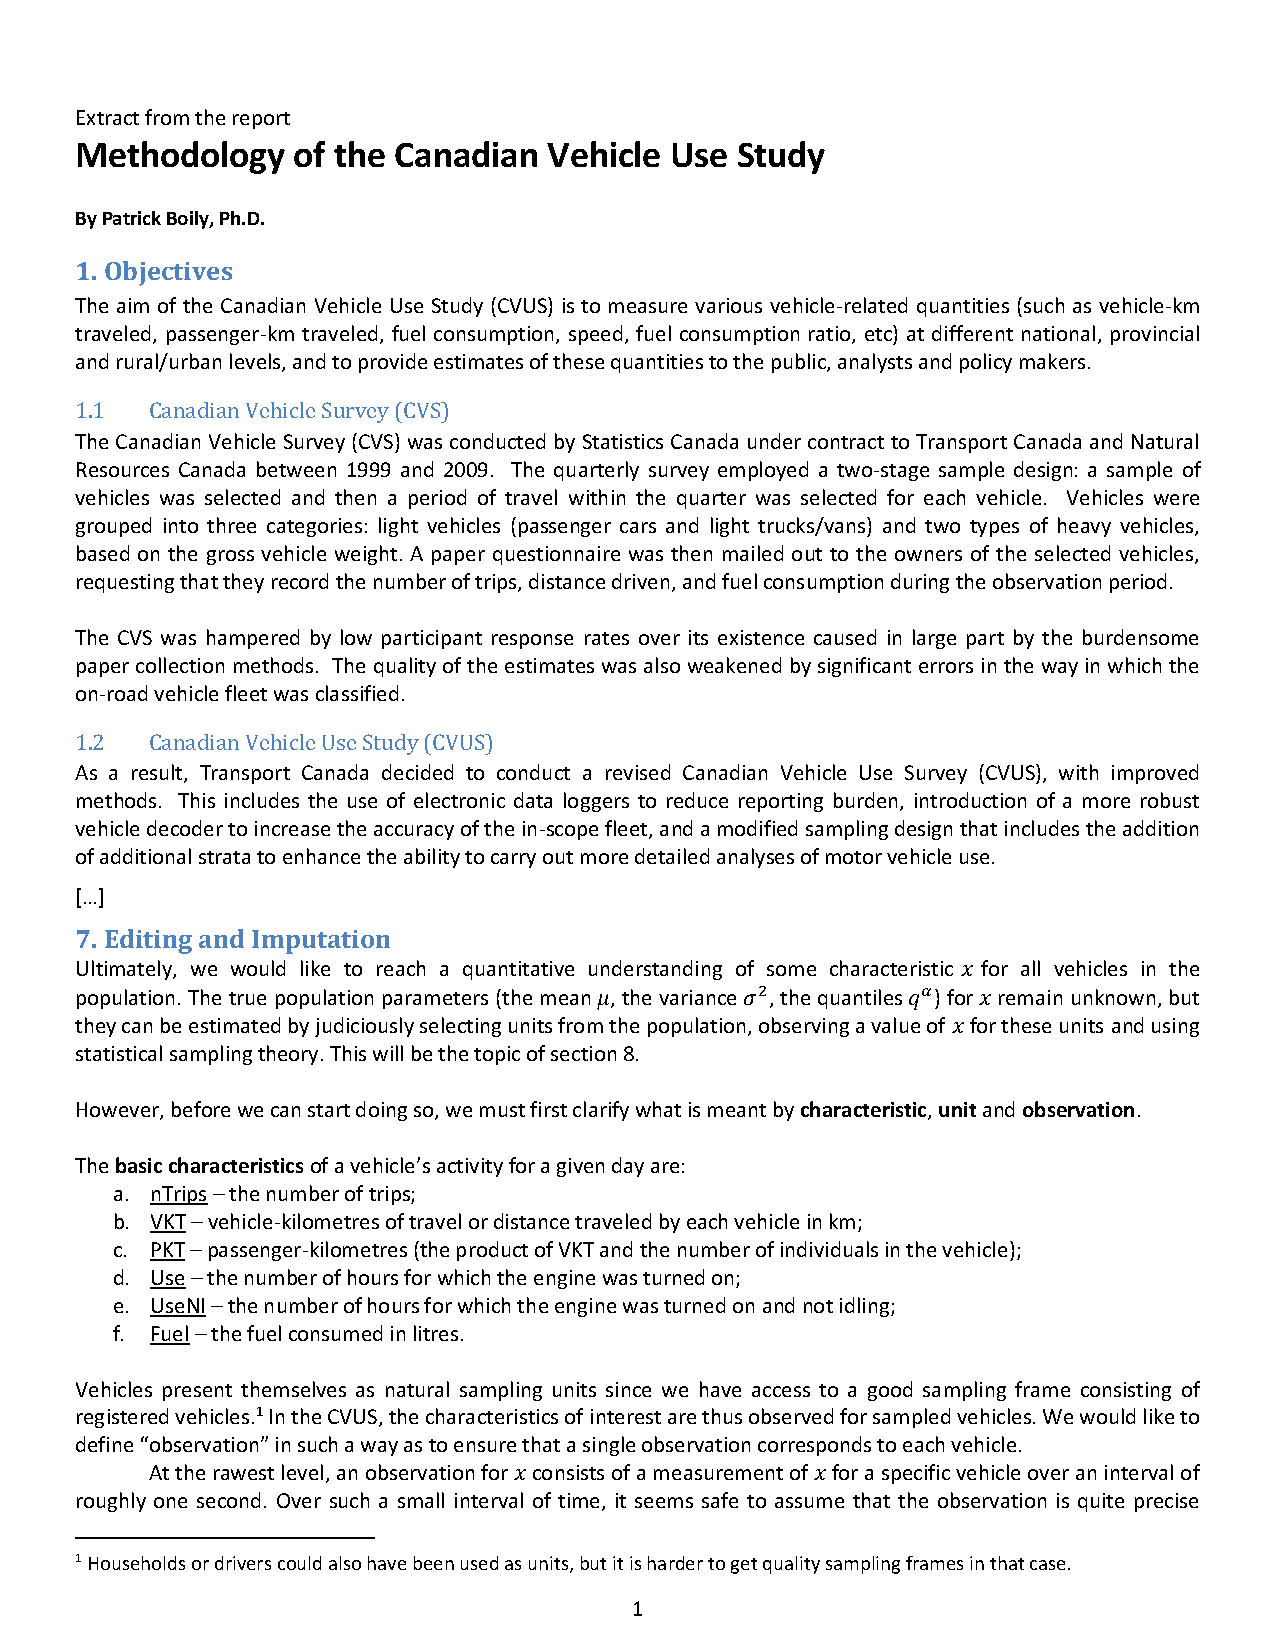
\includepdf[pages={1-10},offset={50 -40}]{documents/CVUS(Extract).pdf}
\includepdf[pages={9-12},offset={50 -40}]{documents/CVUS_Q1_2012_Estimates.pdf}
\setboolean{@twoside}{true}
